% !TeX spellcheck = cs_CZ

\chapter{Úvod}
\label{chap:uvod}

\setcounter{page}{1}
\section{Specifikace}
Program simuluje Sluneční soustavu za využití Newtonova gravitačního zákona a numerických metod. Fyzikálně se jedná řešení problému n-těles - tzn. každé těleso gravitačně působí na všechna ostatní. Tento problém je velmi těžko řešitelný analytickým metodami pro větší n. Výpočetní síla počítačů a numerické metody tak nabízí alternativní řešení tohoto problému.

Vstupem programu jsou strukturovaná data uložená v textovém souboru, která definují fyzikální vlastnosti simulované soustavy, což případně dovoluje snadné změny v zadání. 

Výstup je 2D grafická reprezentace simulované soustavy v reálném čase. Uživatelské rozhraní dovoluje plynule měnit rychlost a přesnost simulace. Dále zobrazuje užitečné informace, jako jsou aktuální pozice a rychlosti pro každý simulovaný objekt vzhledem k jiným objektům. Celou simulaci je také možné nahrát a poté kdykoliv přehrát pomocí zabudovaného přehrávače.

Při vývoji programu byl kladen co největší důraz na pozdější rozšířitelnost. Výsledný program tedy poskytuje několik simulačních metod a lze lehce rozšířit o další metody, popřípadě vstupy/výstupy.

\section{Teorie}
\subsection{Analytický popis}
Newtonův Gravitační zákon (NGZ) popisuje vzájemné silové působení $ {F}_g $ dvou hmotných bodů - Myšlené těleso, kde jeho veškerá hmotnost je soustředěna do jednoho místa. Kde výsledná síla je přitažlivá a $ m_1,m_2 $ jsou hmotnosti obou bodů a $ \boldsymbol{x_1,x_2} $ jejich polohy.

\begin{equation}
	{F}_g= \kappa \dfrac{m_1 m_2}{(\boldsymbol{x_1 - x_2})^2} 
\end{equation}


Simulované objekty(hvězdy, planety, měsíce...) budeme dále pokládat za hmotné body, což je vzhledem k jejich rozměrům a vzdálenostem mezi nimi rozumná aproximace.

Nyní nám NGZ spolu s principem superpozice
\footnote{Princip superpozice říká, že výsledné silové účinky na těleso jsou dány součtem všech sil, které na něj působí.}
 a Newtonovým Zákonem síly \eqref{eq:sila} dává pro $ n $ těles následující soustavu \eqref{eq:soustava} $ n $ obyčejných diferenciálních rovnic. 
 Kde neznámé $ \boldsymbol {x}_i, \boldsymbol{\ddot x}_i $ jsou vektory polohy, resp. zrychlení simulovaných těles. Mínus je zde kvůli přitažlivosti výsledné síly.
\begin{equation}
F= m  \boldsymbol {\ddot x}
\label{eq:sila}
\end{equation}
\begin{align}\label{eq:soustava}
\boldsymbol {\ddot x}_i(t)  = -\kappa \sum_{j=1,j \neq i}^{n}\dfrac{m_i\left( \boldsymbol{x_i}(t) - \boldsymbol{x_j}(t)\right)}
{\left( \boldsymbol{x_i}(t) - \boldsymbol{x_j}(t)\right) ^3} . 
\quad \text{pro } i=1 \dots n
\end{align}

Analytické řešení této soustavy rovnic by nám dalo možnost zjistit polohu, rychlost a zrychlení libovolného simulovaného objektu v libovolném čase na základě počátečních podmínek. Ovšem vyřešit tuto soustavu je pro $ n=>3 $ velmi těžké.

\subsection{Numerické řešení}
\label{sec:numReseni}
Pokud se soustava nedá vyřešit analyticky, můžeme se alespoň pokusit získat aproximativní řešení. Numerické metody využívají toho, že nemusí být tak těžké spočítat derivace v libovolném čase. Navíc to dnešní počítače dokáží udělat velmi rychle. Pokud tedy dokážeme zjistit derivaci v každém bodě, tak bychom mohli původní funkci zrekonstruovat pomocí těchto derivací. Např. můžeme výslednou funkci aproximovat úsečkami, kde jejich směrnice je derivace hledané funkce. Toto přesně dělá nejjednodušší numerická metoda - Eulerova explicitní metoda\eqref{eq:euler}.
Mějme jednoduchou soustavu rovnic \eqref{eq:ex} . Je vidět, že řešením je funkce $ y=e^t $, což se případně snadno ověří zpětnou derivací. 
\begin{align} \label{eq:euler}
y(t+\Delta t) = y(t) + \Delta t . y'(t)
\end{align}
\begin{align} \label{eq:ex}
\dot	y = y, y(0)=1
\end{align}
Zkusme tuto rovnici vyřešit numericky Eulerovou metodou \eqref{eq:euler}. 
Výsledné hodnoty pro různé  $ \Delta t $ jsou vykresleny na obrázku \ref{fig:euler} spolu s analytickým řešením.
Pro dostatečně malá  $ \Delta t $ dostáváme relativně přesné řešení.

Eulerova metoda se dá použít i k řešení naší soustavy \eqref{eq:soustava}, což je podrobněji popsáno u její implementace v sekci \ref{sec:explEuler}. Také další  metody - semi-implicitní Euler a RK4 jsou popsány u svých implementací \ref{sec:implEuler} resp. \ref{sec:implRK4}. Kapitola \ref{chap:compMethods} pak nabízí srovnání těchto metod pro řešení naší soustavy.

\begin{figure}[p]
	\caption{Srovnání různých $ \Delta t $ pro přesnost Eulerovy metody}
	\label{fig:euler}
	\centering
	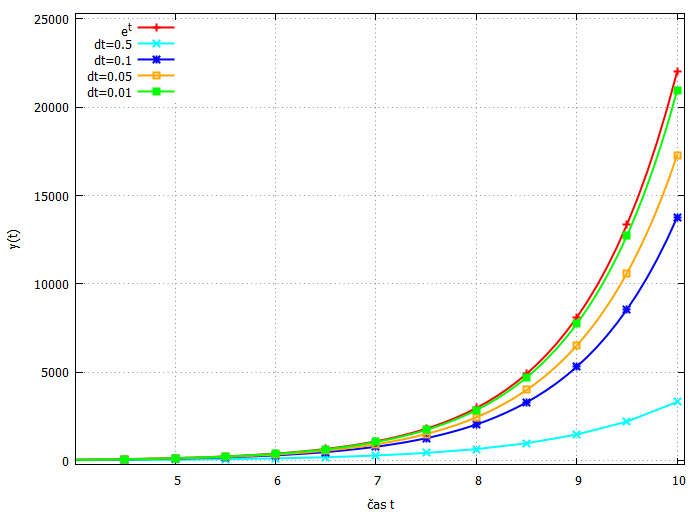
\includegraphics[width=\linewidth]{Figs/eulerTable}
\end{figure}









